% Cross-temporal generalization heatmap (pgfplots, no external images)
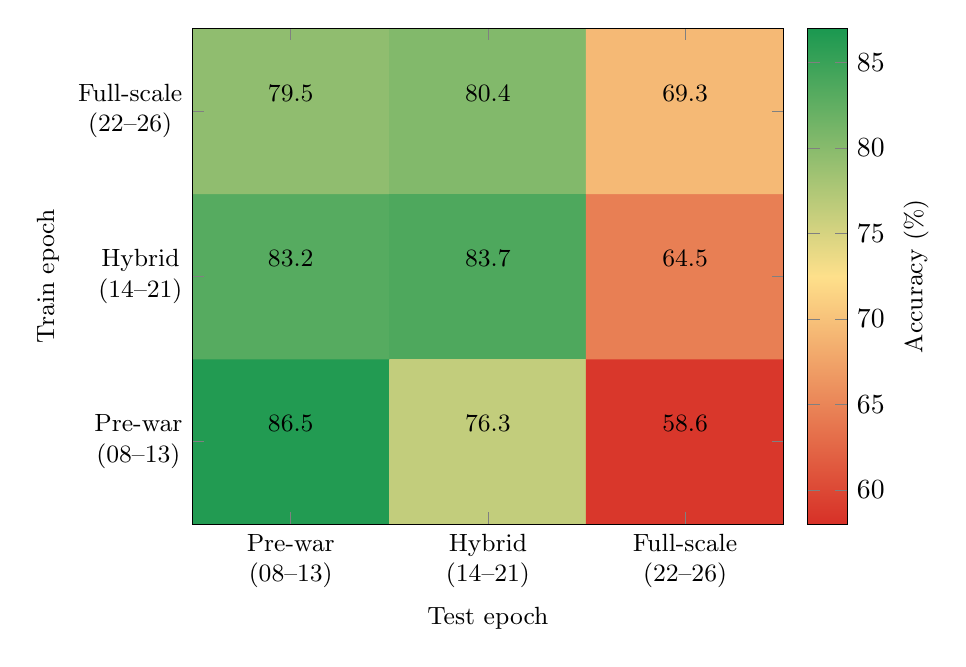
\begin{tikzpicture}
\begin{axis}[
    width=0.75\columnwidth,
    height=0.65\columnwidth,
    colormap={temporal}{
        rgb255(0cm)=(215,48,39);
        rgb255(1cm)=(254,224,139);
        rgb255(2cm)=(26,152,80)
    },
    colorbar,
    colorbar style={
        ylabel={Accuracy (\%)},
        ylabel style={font=\small},
        ytick={60,65,70,75,80,85},
    },
    point meta min=58,
    point meta max=87,
    xtick={0,1,2},
    xticklabels={Pre-war\\(08--13), Hybrid\\(14--21), Full-scale\\(22--26)},
    ytick={0,1,2},
    yticklabels={Pre-war\\(08--13), Hybrid\\(14--21), Full-scale\\(22--26)},
    x tick label style={align=center, font=\small},
    y tick label style={align=center, font=\small},
    xlabel={Test epoch},
    ylabel={Train epoch},
    xlabel style={font=\small},
    ylabel style={font=\small},
    enlargelimits=false,
    axis on top,
    nodes near coords={\pgfmathprintnumber\pgfplotspointmeta},
    every node near coord/.append style={font=\small\bfseries, black},
]
\addplot[matrix plot*, mesh/cols=3, mesh/rows=3, point meta=explicit]
    coordinates {
        (0,0) [86.5]  (1,0) [76.3]  (2,0) [58.6]
        (0,1) [83.2]  (1,1) [83.7]  (2,1) [64.5]
        (0,2) [79.5]  (1,2) [80.4]  (2,2) [69.3]
    };
\end{axis}
\end{tikzpicture}
